In the following diagram, the mentioned components are more closely examined, with the main focus on the application server. While describing the parts, the notation will be the interface they are providing in order to be more general, because there may be one or more different implementations of the same service within the server. The components shown here communicate with each other and work together to complete certain user requests.\newline\newline
\textbf{DATA4HELP SERVICE}
\begin{figure}[H]
	\begin{center}
		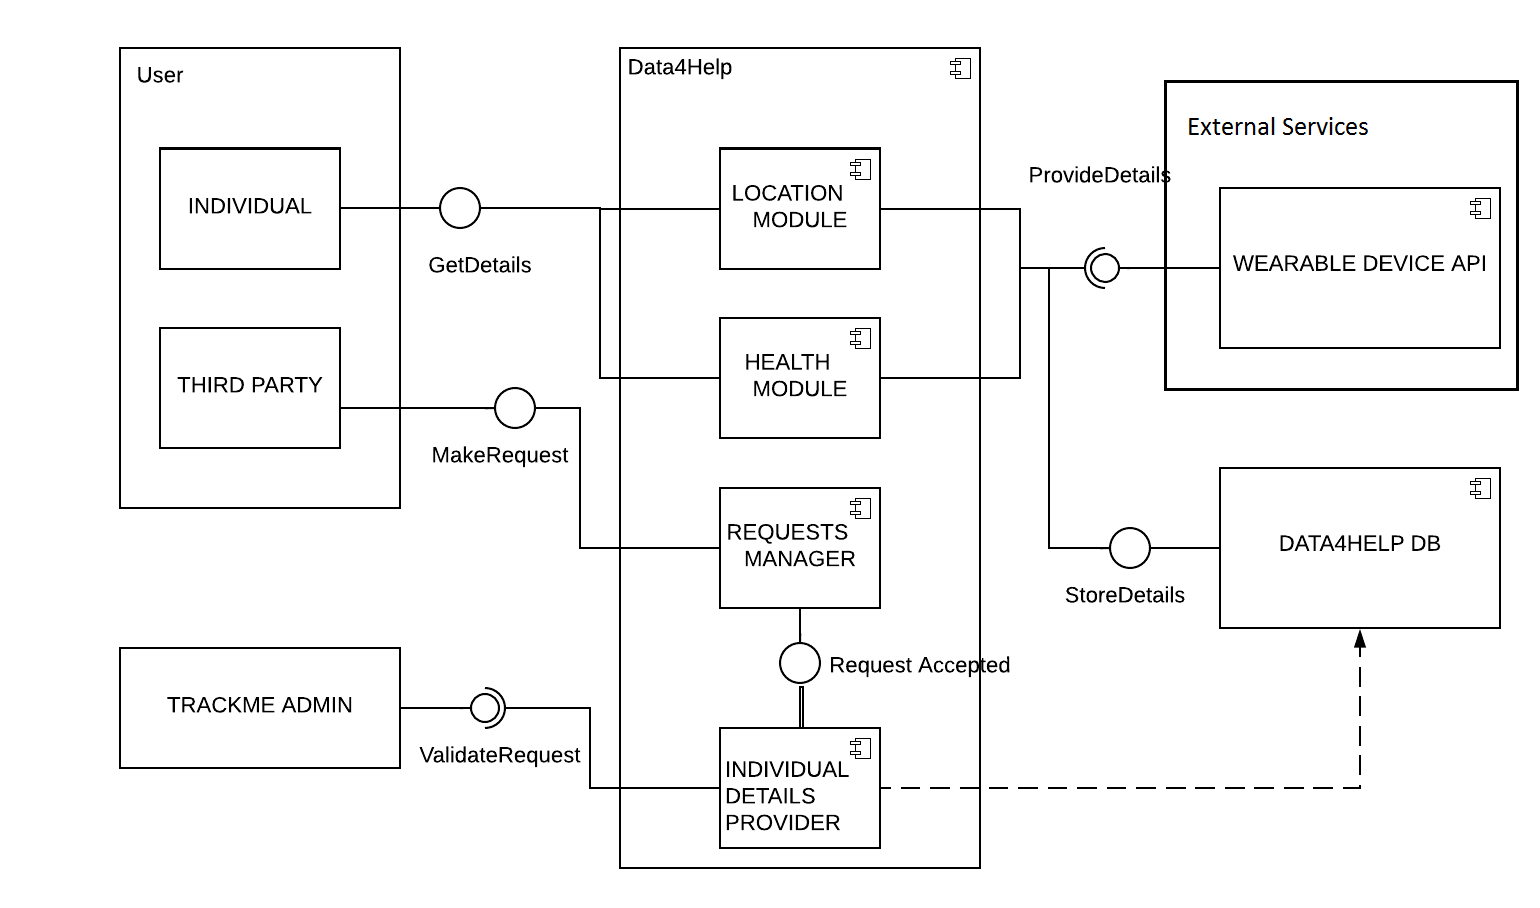
\includegraphics[width=\textwidth]{./DD_Diagrams/ComponentData4Help.png}
      	\caption{Component Diagram for Data4Help Service}
        \label{TrackMe_c1}
	\end{center}
\end{figure}

\begin{itemize}
\item\textbf{Location module:}  the location fetched from the Wearable Device API provided by an Individual is stored in the Data4Help DB.
\item\textbf{Health module:}  the health values fetched from the Wearable Device API provided by an Individual is stored in the Data4Help DB.
\item\textbf{Request Manager:}  provides an interface to the Third Party to make new request to get the details of a specific Individual or a group of Individual. It also provides an interface to a specific Individual to accept or reject the request.
\item\textbf{Individual Details Provider:} this uses the  help of the Data4Help DB to provide the details to the Third Party after the TrackMe Admin has validated the request.
\newline
\end{itemize}
\textbf{AUTOMATEDSOS SERVICE}
\begin{figure}[H]
	\begin{center}
		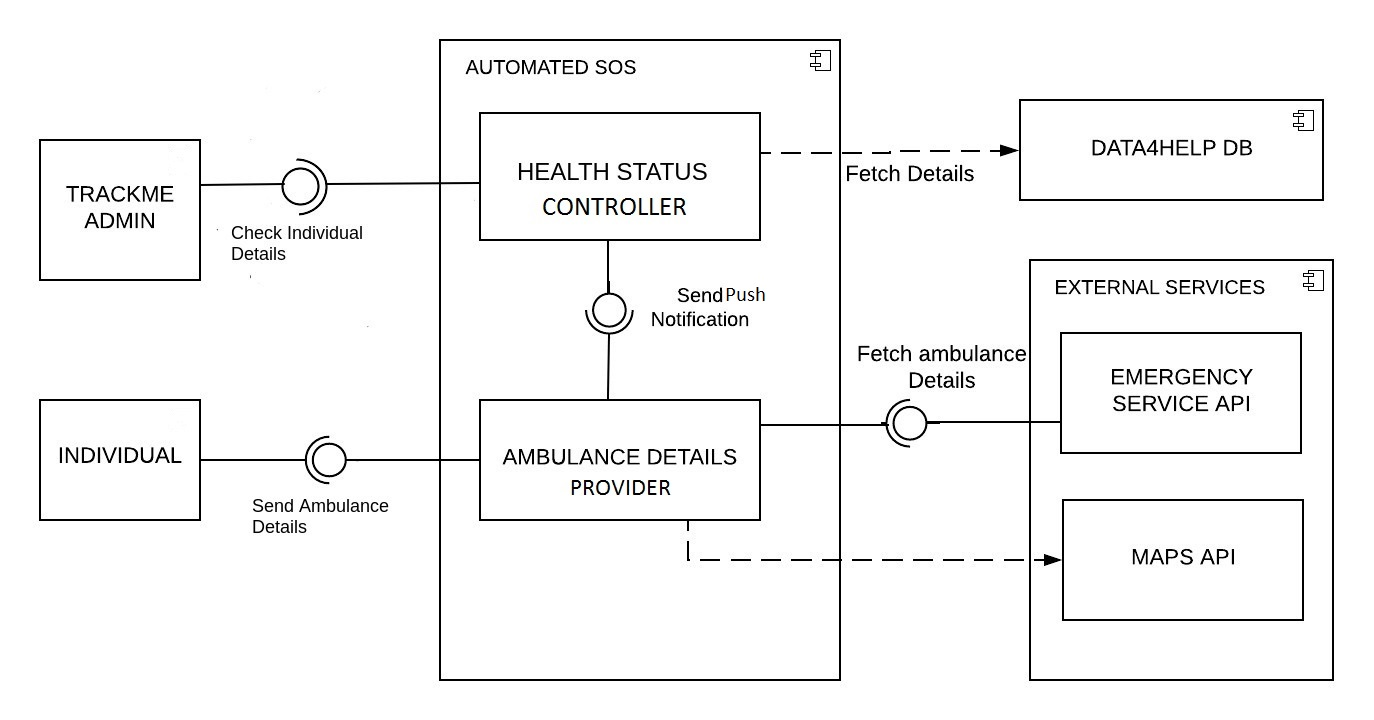
\includegraphics[width=\textwidth]{./DD_Diagrams/ComponentAutomatedSOS.jpg}
      	\caption{Component Diagram for AutomatedSOS Service}
        \label{TrackMe_c2}
	\end{center}
\end{figure}

\begin{itemize}
\item\textbf{Health Status Controller:}  uses the help of the Data4Help DB to get the details of an Individual. The TrackMe Admin provides an interface check Individual Details to the controller. The controller then, monitors the individual's vitals and when the vital is below the threshold value, it provides an interface named send notification.  
\item\textbf{Ambulance Details Provider:} gets the details of all the Ambulance associated to the major hospitals from the Emergency Service API. It uses the maps API to get the nearby ambulances and send notification to that ambulance driver application. It uses the functionality of Push Notification to send the notification. After a driver accept the request, the details of the driver is send to the Individual. 
\newline
\end{itemize}
\textbf{TRACK4RUN SERVICE}

\begin{figure}[H]
	\begin{center}
		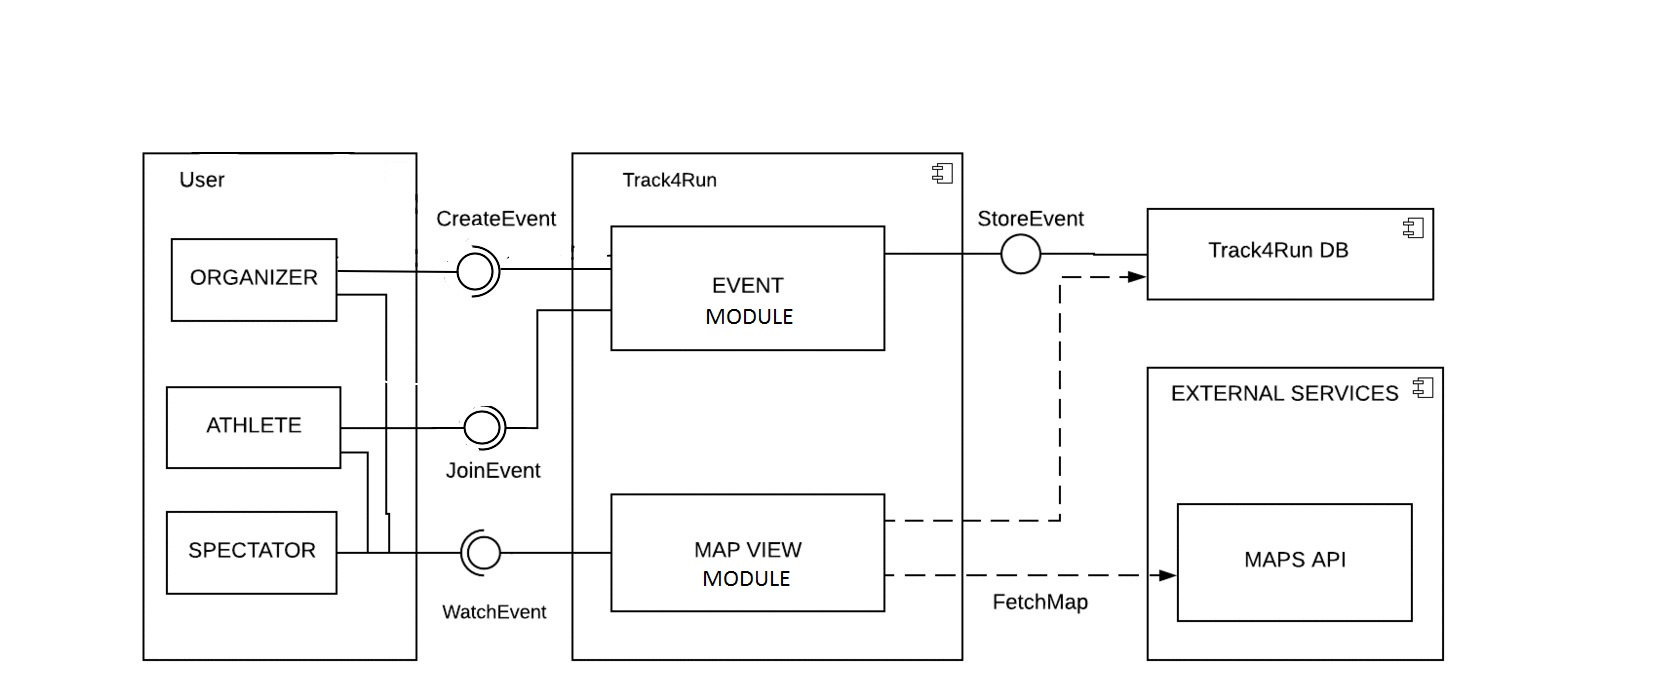
\includegraphics[width=\textwidth]{./DD_Diagrams/ComponentTrack4Run.jpg}
      	\caption{Component Diagram for Track4Run Service}
        \label{TrackMe_c3}
	\end{center}
\end{figure}

\begin{itemize}
\item\textbf{Event Module:} manages the details of the event and the athletes. It gets all the details of the event from the organizer which is entered after the organizer upgrades to the service. The event details is stored in the Track4Run DB. The athlete joins the event and is then associated with that specific event. 
\item\textbf{Map View Module:} It uses the Map API to provide an interface watch event to the organizer, athlete and the spectator. It checks the validity of the subscribed users. It uses the Track4Run DB to get the location of the athletes participating in an event, and then maps it to the interface.
\newline\newline\newline\newline\newline
\end{itemize}
\textbf{MAIN COMPONENT}

\begin{figure}[H]
	\begin{center}
		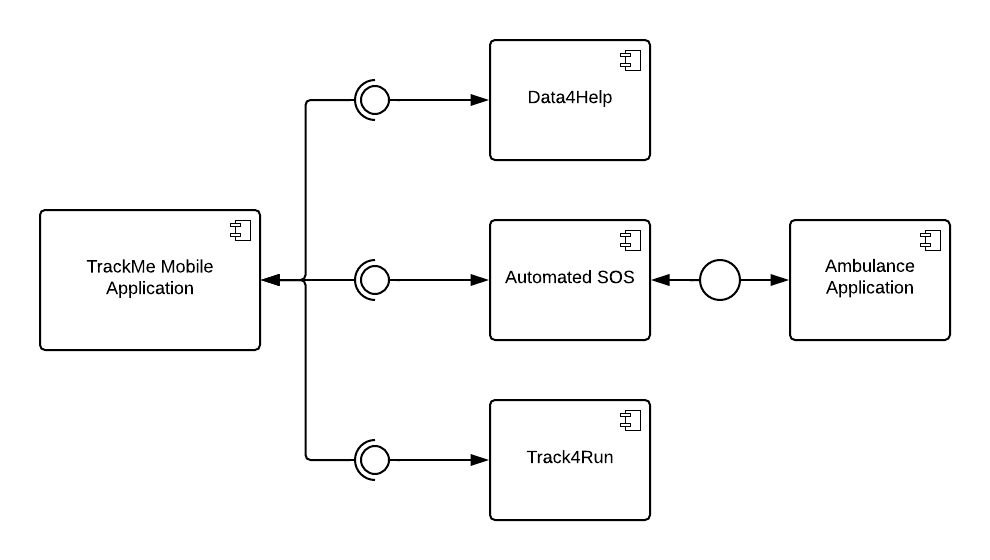
\includegraphics[width=\textwidth]{./DD_Diagrams/Component.png}
      \caption{Main Component Diagram}
        \label{TrackMe_c0}
	\end{center}
\end{figure}
The main component is divided into three subcomponents which are shown separately to avoid unreadability. All the three subcomponents are the services which is being provided by the TrackMe Application.\newline
The Ambulance Application is a separate application developed explicitly for the ambulance drivers where they receive individuals details through push notification. It is connected to Automated SOS service for exchange of information of ambulance and individual respectively.